\documentclass[a4paper, 12pt]{article}

%%% Работа с русским языком
\usepackage{cmap}					% поиск в PDF
\usepackage{mathtext} 				% русские буквы в формулах
\usepackage[T2A]{fontenc}			% кодировка
\usepackage[utf8]{inputenc}			% кодировка исходного текста
\usepackage[russian]{babel}	% локализация и переносы

%%% Дополнительная работа с математикой
\usepackage{amsmath,amsfonts,amssymb,amsthm,mathtools} % AMS
\usepackage{icomma} % "Умная" запятая: $0,2$ --- число, $0, 2$ --- перечисление

%% Номера формул
%\mathtoolsset{showonlyrefs=true} % Показывать номера только у тех формул, на которые есть \eqref{} в тексте.

%% Шрифты
\usepackage{euscript}	 % Шрифт Евклид
\usepackage{mathrsfs} % Красивый матшрифт

%% Поля
\usepackage[left=2cm,right=2cm,top=2cm,bottom=2cm,bindingoffset=0cm]{geometry}

%% Русские списки
\usepackage{enumitem}
\makeatletter
\AddEnumerateCounter{\asbuk}{\russian@alph}{щ}
\makeatother

%%% Работа с картинками
\usepackage{graphicx}  % Для вставки рисунков
\graphicspath{{images/}{images2/}}  % папки с картинками
\setlength\fboxsep{3pt} % Отступ рамки \fbox{} от рисунка
\setlength\fboxrule{1pt} % Толщина линий рамки \fbox{}
\usepackage{wrapfig} % Обтекание рисунков и таблиц текстом

%%% Работа с таблицами
\usepackage{array,tabularx,tabulary,booktabs} % Дополнительная работа с таблицами
\usepackage{longtable}  % Длинные таблицы
\usepackage{multirow} % Слияние строк в таблице

%% Красная строка
\setlength{\parindent}{2em}

%% Интервалы
\linespread{1}
\usepackage{multirow}

%% TikZ
\usepackage{tikz}
\usetikzlibrary{graphs,graphs.standard}

%% Верхний колонтитул
\usepackage{fancyhdr}
\pagestyle{fancy}

%% Перенос знаков в формулах (по Львовскому)
\newcommand*{\hm}[1]{#1\nobreak\discretionary{}
	{\hbox{$\mathsurround=0pt #1$}}{}}

%% Мои дополнения
\usepackage{float} %Добавляет возможность работы с командой [H] которая улучшает расположение на странице
\usepackage{gensymb} %Красивые градусы
\usepackage{graphicx}               % Импорт изображений
\usepackage{caption} % Пакет для подписей к рисункам, в частности, для работы caption*

% подключаем hyperref (для ссылок внутри  pdf)
\usepackage[unicode, pdftex]{hyperref}

%%% Теоремы
\theoremstyle{plain}                    % Это стиль по умолчанию, его можно не переопределять.
\renewcommand\qedsymbol{$\blacksquare$} % переопределение символа завершения доказательства

\newtheorem{theorem}{Теорема}[section] % Теорема (счетчик по секиям)
\newtheorem{proposition}{Утверждение}[section] % Утверждение (счетчик по секиям)
\newtheorem{definition}{Определение}[section] % Определение (счетчик по секиям)
\newtheorem{corollary}{Следствие}[theorem] % Следстиве (счетчик по теоремам)
\newtheorem{problem}{Задача}[section] % Задача (счетчик по секиям)
\newtheorem*{remark}{Примечание} % Примечание (можно переопределить, как Замечание)
\newtheorem{lemma}{Лемма}[section] % Лемма (счетчик по секиям)

\begin{document}
    \newcommand{\HRule}{\rule{\linewidth}{0.7mm}} % Defines a new command for the horizontal lines, change thickness here
	
	\begin{center}
		\large\textbf{Московский Физико-Технический Институт}\\ % Name of your university/college
		\large\textbf{(государственный университет)}
	
		\vfill
		
		\Large Лабораторная работа по курсу общей физики № *labnum*\\[0.5cm] % Preambule of your document title
		
		
		\HRule
		\\[0.4cm]
		{ \huge \bfseries *name of your labwork*}% Title of your document
		\\[0.4cm] 
		\HRule
		\\[0.5cm]
		
		\ \\
	\textbf{\large Автор:} \\	
	\large *your name* *groupname*\\ % Your name and something more, your group num for example
		\vfill
		\hspace*{-0.8 cm}
\includegraphics[width=100 pt]{frkt_logo}\\ % logo of your  company/university/college
		\large Долгопрудный, 2021 % location and year
	\end{center}

\newpage
\setcounter{page}{2}
\fancyfoot[c]{\thepage}
\fancyhead[L] {Работа № *labnum*} % some information in page header
\fancyhead[R]{}

    \section*{Цель работы}
    Методом электронного возбуждения измерить энергию первого уровня атома гелия в динамическом и статическом режимах.

    \section*{Теоретические сведения}

    Разреженный одноатомный газ (в нашем случае -- гелий) заполняет трёхэлектродную лампу. Электроны, испускаемые разогретым катодом, ускоряются в постоянном электрическом поле, созданным между катодом и сетчатым анодом лампы. Передвигаясь от катода к аноду, электроны сталкиваются с атомами гелия. Если энергия электрона, налетающего на атом, недостаточна для того, чтобы перевести его в возбуждённое состояние (или ионизовать), то возможны только упругие соударения, при которых электроны почти не теряют энергии, так как их масса в тысячи раз меньше массы атомов.


    По мере увеличения разности потенциалов между анодом и катодом энергия электронов увеличивается и, в конце концов, оказывается достаточной для возбуждения атомов. При таких -- неупругих -- столкновениях кинетическая энергия налетающего электрона передаётся одному из атомных электронов, вызывая его переход на свободный энергетический уровень (возбуждение) или совсем отрывая его от атома (ионизация).

    При увеличении потенциала анода ток в лампе вначале растёт, подобно тому как это происходит в вакуумном диоде (рис. 2). Однако, когда энергия электронов становится достаточной для возбуждения атомов, ток коллектора резко уменьшается. Это происходит потому, что при неупругих соударениях с атомами электроны почти полностью теряют свою энергию и не могут преодолеть задерживающего потенциала между анодом и коллектором. При дальнейшем увеличении потенциала анода ток коллектора вновь возрастает: электроны, испытавшие неупругие соударения, при дальнейшем движении к аноду успевают набрать энергию, достаточную для преодоления задерживающего потенциала.


    \begin{figure}[h!]
        \centering
        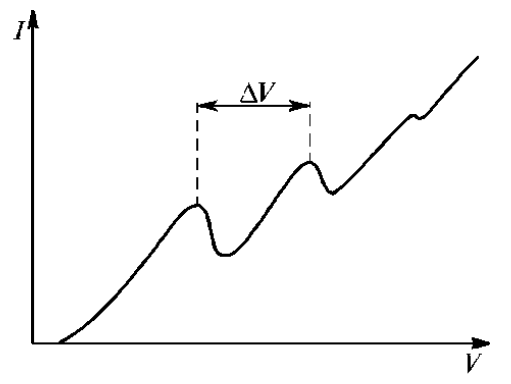
\includegraphics[width=0.4\textheight]{Screenshot_1}
        \caption{Характер зависимости $I (U)$}
        \label{fig:screenshot1}
    \end{figure}

    \section*{Оборудование}

    Схема экспериментальной установки отображена на рис. \ref{fig:screenshot2} и \ref{fig:screenshot3}.

    \begin{figure}[tbh]
        \centering
        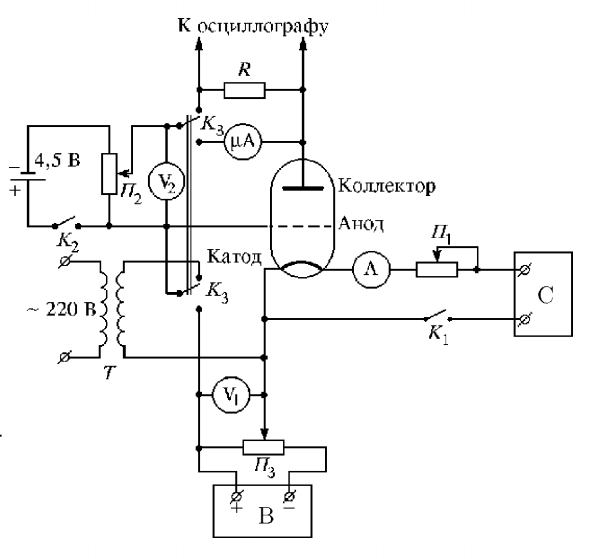
\includegraphics[height=0.4\textheight]{Screenshot_2}
        \caption{Принципиальная схема установки}
        \label{fig:screenshot2}
    \end{figure}

    \begin{figure}[tbh]
        \centering
        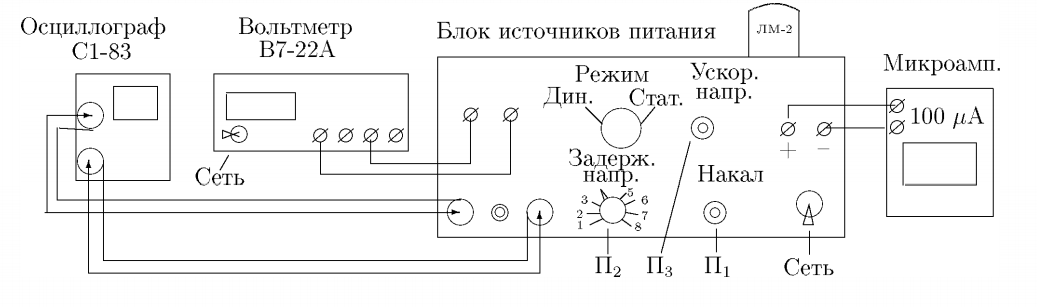
\includegraphics[width=0.6\textheight]{Screenshot_3}
        \caption{Блок-схема экспериментальной установки}
        \label{fig:screenshot3}
    \end{figure}

    \section*{Задача о потенциальной яме}

    Решим задачу о частице в потенциальной яме. Найдем разрешенные уровни энергии частицы
    в потенциальной яме с бесконечновысокими стенками.

    \begin{figure}[tbh]
        \centering
        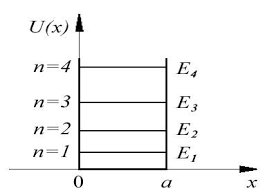
\includegraphics[width=0.3\textheight]{potential_pit.png}
        \caption{Потенциальная яма}
        \label{fig:potential_pit}
    \end{figure}


    \section*{Обработка данных}

    В динамическом режиме получили на экране осцилогрфа инвертированную вольт-амперную характиристику.

    \begin{figure}[h]
        \centering
        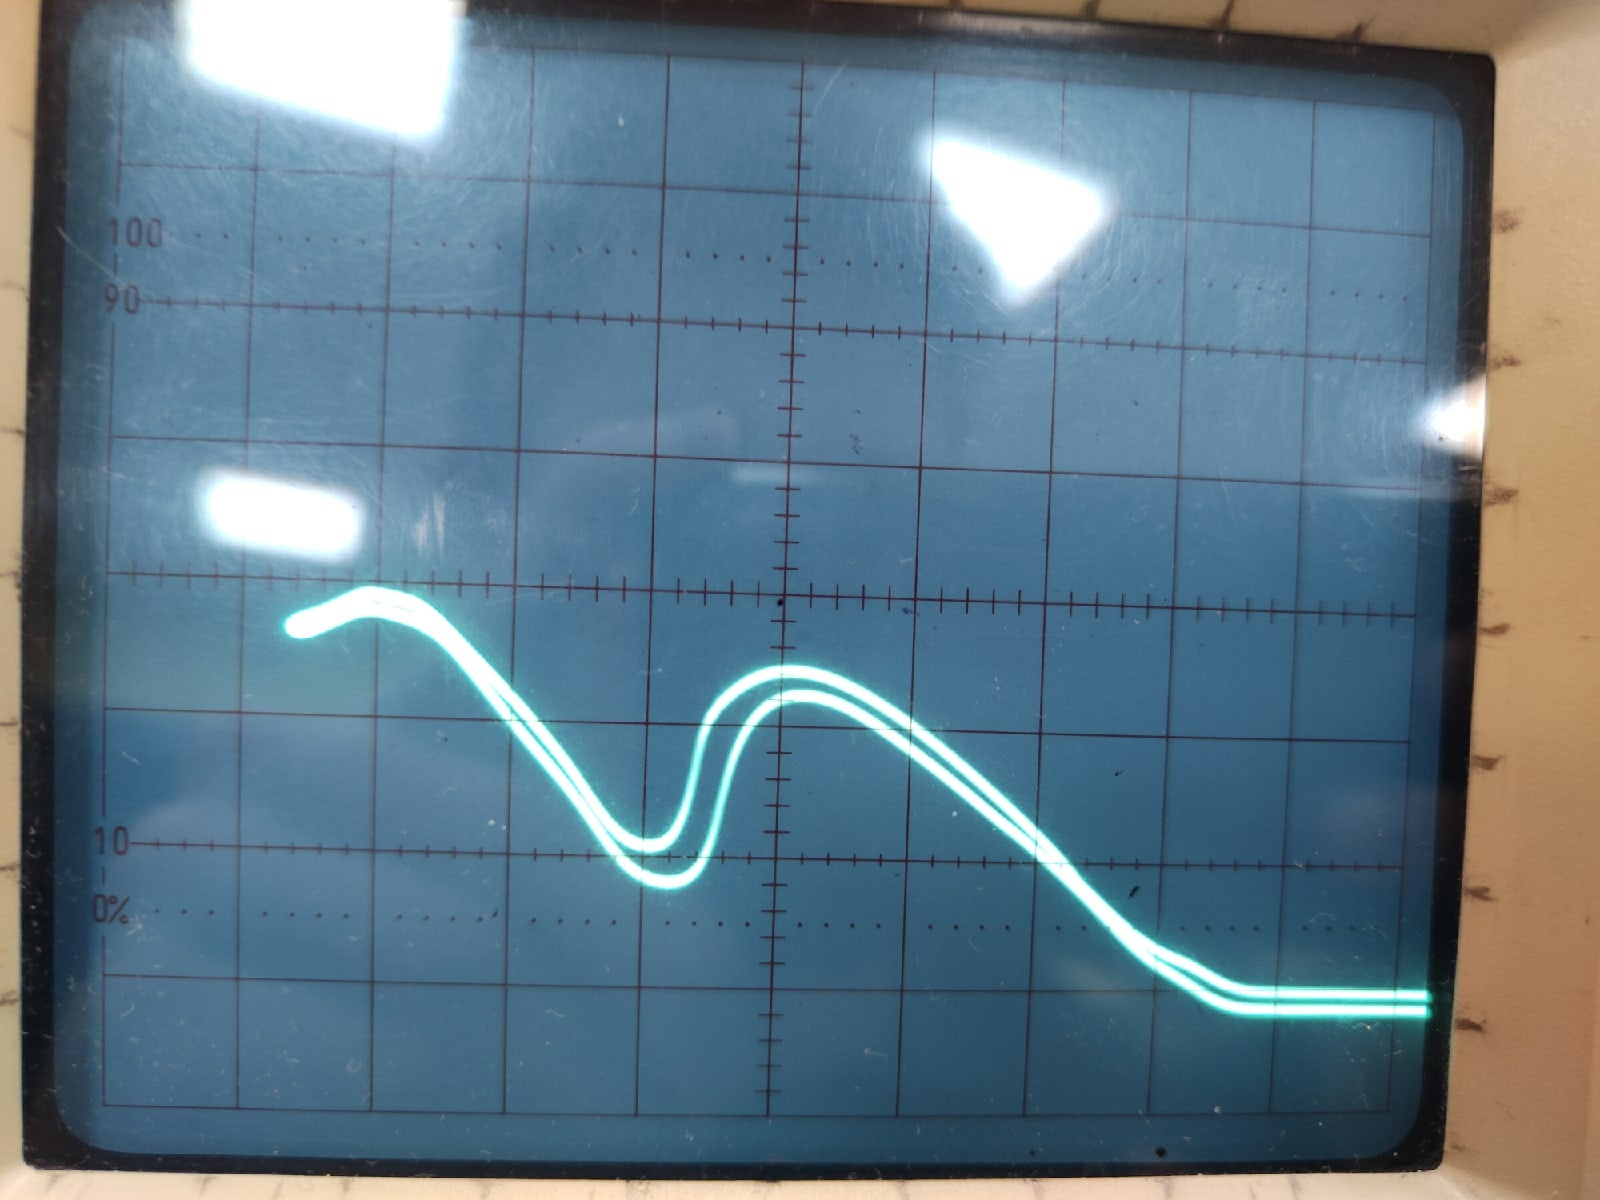
\includegraphics[width=0.6\textheight]{1}
        \caption{Вольтамперная характиристика, полученная в динамическом режиме}
        \label{fig:1}
    \end{figure}

    Цена деления по горизонтали 5 В. Таким образом, интервал напряжения между соседними пиками порядка 15 В.
    Точное значение интервала между пиками установить по осцилографу сложно. Данный этап дает лишь оценочное значение.

    В статическом режиме снимим вольт-амперную характиристику при значениях запирающего напряжения 4 В, 6 В и 9 В.

    \begin{table}[]
    \centering
    \begin{tabular}{|ll|ll|ll|}
    \hline
    \multicolumn{2}{|l|}{4 В}                                      & \multicolumn{2}{l|}{6 В}                                     & \multicolumn{2}{l|}{9 В}                                     \\ \hline
    \multicolumn{1}{|l|}{V$\pm 0.01$, В}    & I $\pm 0.001$ мА     & \multicolumn{1}{l|}{V$\pm 0.01$, В}    & I $\pm 0.001$ мА    & \multicolumn{1}{l|}{V$\pm 0.01$, В}    & I $\pm 0.001$ мА    \\ \hline
    \multicolumn{1}{|l|}{4.25}              & 0.062                & \multicolumn{1}{l|}{2.60}              & 0.019               & \multicolumn{1}{l|}{5.28}              & 0.015               \\ \hline
    \multicolumn{1}{|l|}{6.25}              & 0.094                & \multicolumn{1}{l|}{6.05}              & 0.066               & \multicolumn{1}{l|}{10.0}              & 0.090               \\ \hline
    \multicolumn{1}{|l|}{8.14}              & 0.127                & \multicolumn{1}{l|}{9.12}              & 0.120               & \multicolumn{1}{l|}{12.6}              & 0.133               \\ \hline
    \multicolumn{1}{|l|}{10.8}              & 0.171                & \multicolumn{1}{l|}{12.3}              & 0.169               & \multicolumn{1}{l|}{14.9}              & 0.167               \\ \hline
    \multicolumn{1}{|l|}{14.6}              & 0.223                & \multicolumn{1}{l|}{16.0}              & 0.221               & \multicolumn{1}{l|}{17.4}              & 0.203               \\ \hline
    \multicolumn{1}{|l|}{17.5}              & 0.258                & \multicolumn{1}{l|}{16.7}              & 0.228               & \multicolumn{1}{l|}{19.5}              & 0.228               \\ \hline
    \multicolumn{1}{|l|}{17.9}              & 0.262                & \multicolumn{1}{l|}{17.4}              & 0.239               & \multicolumn{1}{l|}{20.7}              & 0.235               \\ \hline
    \multicolumn{1}{|l|}{18.7}              & 0.269                & \multicolumn{1}{l|}{18.1}              & 0.249               & \multicolumn{1}{l|}{21.6}              & 0.236               \\ \hline
    \multicolumn{1}{|l|}{19.7}              & 0.274                & \multicolumn{1}{l|}{19.1}              & 0.258               & \multicolumn{1}{l|}{22.5}              & 0.233               \\ \hline
    \multicolumn{1}{|l|}{21.0}              & 0.274                & \multicolumn{1}{l|}{20.0}              & 0.263               & \multicolumn{1}{l|}{24.0}              & 0.203               \\ \hline
    \multicolumn{1}{|l|}{21.9}              & 0.271                & \multicolumn{1}{l|}{21.0}              & 0.263               & \multicolumn{1}{l|}{24.3}              & 0.183               \\ \hline
    \multicolumn{1}{|l|}{22.3}              & 0.261                & \multicolumn{1}{l|}{21.9}              & 0.257               & \multicolumn{1}{l|}{24.5}              & 0.098               \\ \hline
    \multicolumn{1}{|l|}{22.7}              & 0.251                & \multicolumn{1}{l|}{22.5}              & 0.252               & \multicolumn{1}{l|}{25.2}              & 0.078               \\ \hline
    \multicolumn{1}{|l|}{23.0}              & 0.221                & \multicolumn{1}{l|}{23.2}              & 0.236               & \multicolumn{1}{l|}{26.5}              & 0.071               \\ \hline
    \multicolumn{1}{|l|}{23.3}              & 0.211                & \multicolumn{1}{l|}{23.4}              & 0.221               & \multicolumn{1}{l|}{27.6}              & 0.077               \\ \hline
    \multicolumn{1}{|l|}{24.3}              & 0.213                & \multicolumn{1}{l|}{23.5}              & 0.205               & \multicolumn{1}{l|}{28.8}              & 0.093               \\ \hline
    \multicolumn{1}{|l|}{24.7}              & 0.218                & \multicolumn{1}{l|}{23.8}              & 0.169               & \multicolumn{1}{l|}{29.6}              & 0.112               \\ \hline
    \multicolumn{1}{|l|}{25.4}              & 0.232                & \multicolumn{1}{l|}{24.8}              & 0.144               & \multicolumn{1}{l|}{30.6}              & 0.138               \\ \hline
    \multicolumn{1}{|l|}{26.3}              & 0.249                & \multicolumn{1}{l|}{25.8}              & 0.152               & \multicolumn{1}{l|}{31.6}              & 0.160               \\ \hline
    \multicolumn{1}{|l|}{26.8}              & 0.259                & \multicolumn{1}{l|}{27.7}              & 0.194               & \multicolumn{1}{l|}{33.8}              & 0.207               \\ \hline
    \multicolumn{1}{|l|}{27.6}              & 0.275                & \multicolumn{1}{l|}{29.0}              & 0.220               & \multicolumn{1}{l|}{35.8}              & 0.240               \\ \hline
    \multicolumn{1}{|l|}{28.5}              & 0.293                & \multicolumn{1}{l|}{29.9}              & 0.240               & \multicolumn{1}{l|}{37.0}              & 0.250               \\ \hline
    \multicolumn{1}{|l|}{29.4}              & 0.309                & \multicolumn{1}{l|}{31.9}              & 0.277               & \multicolumn{1}{l|}{38.6}              & 0.255               \\ \hline
    \multicolumn{1}{|l|}{32.1}              & 0.359                & \multicolumn{1}{l|}{33.4}              & 0.306               & \multicolumn{1}{l|}{39.4}              & 0.253               \\ \hline
    \multicolumn{1}{|l|}{33.8}              & 0.389                & \multicolumn{1}{l|}{35.0}              & 0.333               & \multicolumn{1}{l|}{41.1}              & 0.241               \\ \hline
    \multicolumn{1}{|l|}{35.0}              & 0.409                & \multicolumn{1}{l|}{36.9}              & 0.346               & \multicolumn{1}{l|}{42.9}              & 0.229               \\ \hline
    \multicolumn{1}{|l|}{37.3}              & 0.419                & \multicolumn{1}{l|}{39.0}              & 0.347               & \multicolumn{1}{l|}{44.4}              & 0.218               \\ \hline
    \multicolumn{1}{|l|}{38.5}              & 0.419                & \multicolumn{1}{l|}{40.9}              & 0.330               & \multicolumn{1}{l|}{46.4}              & 0.201               \\ \hline
    \multicolumn{1}{|l|}{39.4}              & 0.411                & \multicolumn{1}{l|}{42.9}              & 0.316               & \multicolumn{1}{l|}{48.2}              & 0.196               \\ \hline
    \multicolumn{1}{|l|}{40.5}              & 0.400                & \multicolumn{1}{l|}{44.5}              & 0.308               & \multicolumn{1}{l|}{50.1}              & 0.192               \\ \hline
    \multicolumn{1}{|l|}{40.9}              & 0.395                & \multicolumn{1}{l|}{46.1}              & 0.305               & \multicolumn{1}{l|}{51.7}              & 0.199               \\ \hline
    \multicolumn{1}{|l|}{41.7}              & 0.391                & \multicolumn{1}{l|}{47.7}              & 0.308               & \multicolumn{1}{l|}{52.7}              & 0.204               \\ \hline
    \multicolumn{1}{|l|}{42.7}              & 0.387                & \multicolumn{1}{l|}{49.4}              & 0.317               & \multicolumn{1}{l|}{}                  &                     \\ \hline
    \multicolumn{1}{|l|}{44.5}              & 0.388                & \multicolumn{1}{l|}{51.6}              & 0.330               & \multicolumn{1}{l|}{}                  &                     \\ \hline
    \multicolumn{1}{|l|}{45.2}              & 0.390                & \multicolumn{1}{l|}{53.1}              & 0.343               & \multicolumn{1}{l|}{}                  &                     \\ \hline
    \multicolumn{1}{|l|}{49.4}              & 0.417                & \multicolumn{1}{l|}{56.0}              & 0.370               & \multicolumn{1}{l|}{}                  &                     \\ \hline
    \end{tabular}
    \caption{Таблица эксперементальных данных для трех запирающих напряжений}
    \label{tab:data}
    \end{table}

    По данных из таблицы \ref{tab:data} для каждого значения запирающего напряжения построим вольльтамперную 
    характиристику.

    \begin{figure}[h]
        \centering
        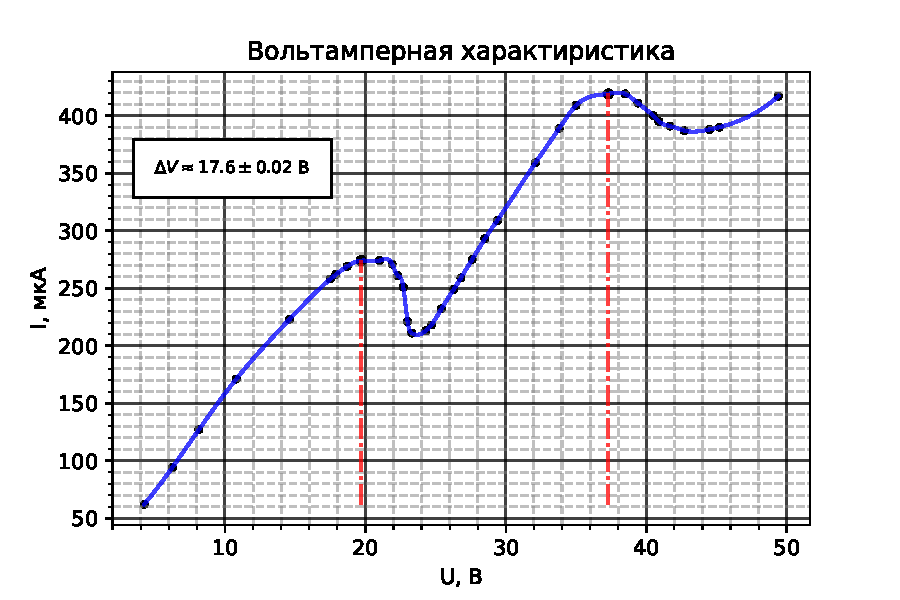
\includegraphics[width=0.6\textheight]{loc_V_4.pdf}
        \caption{ВАХ для запирающего напряжения 4 В}
        \label{fig:loc_V_4}
    \end{figure}

    \begin{figure}[h]
        \centering
        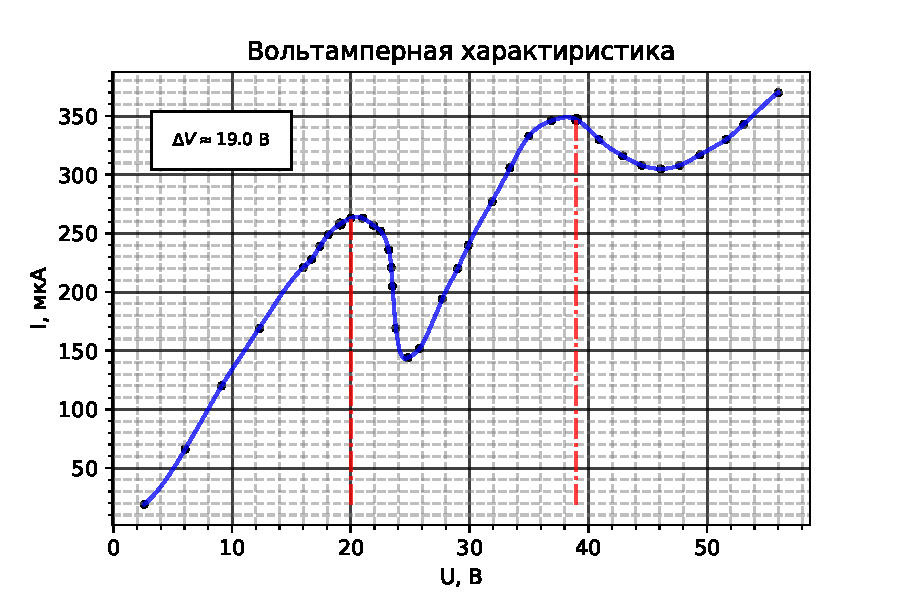
\includegraphics[width=0.6\textheight]{loc_V_6.pdf}
        \caption{ВАХ для запирающего напряжения 6 В}
        \label{fig:loc_V_6}
    \end{figure}

    \begin{figure}[h]
        \centering
        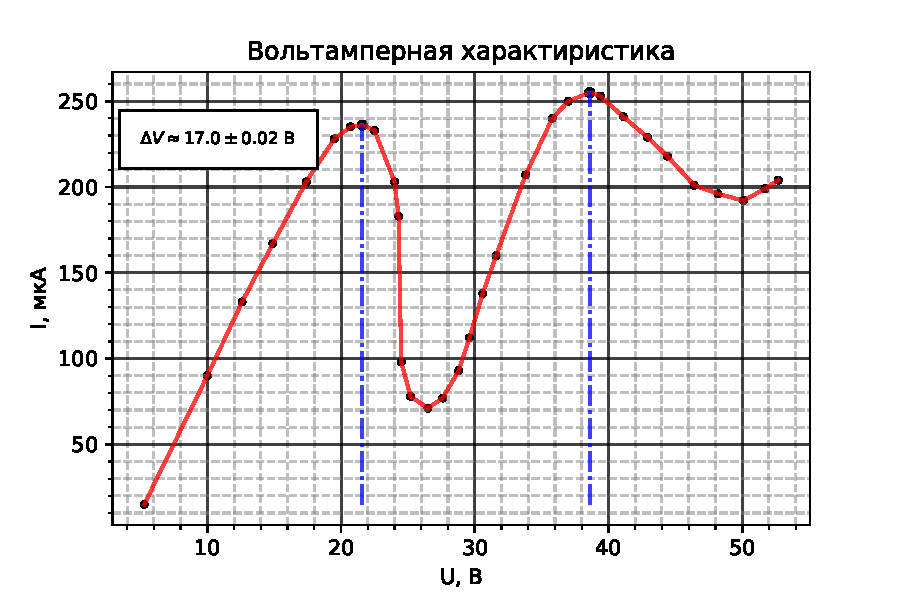
\includegraphics[width=0.6\textheight]{loc_V_9.pdf}
        \caption{ВАХ для запирающего напряжения 9 В}
        \label{fig:loc_V_9}
    \end{figure}

    \begin{figure}[h]
        \centering
        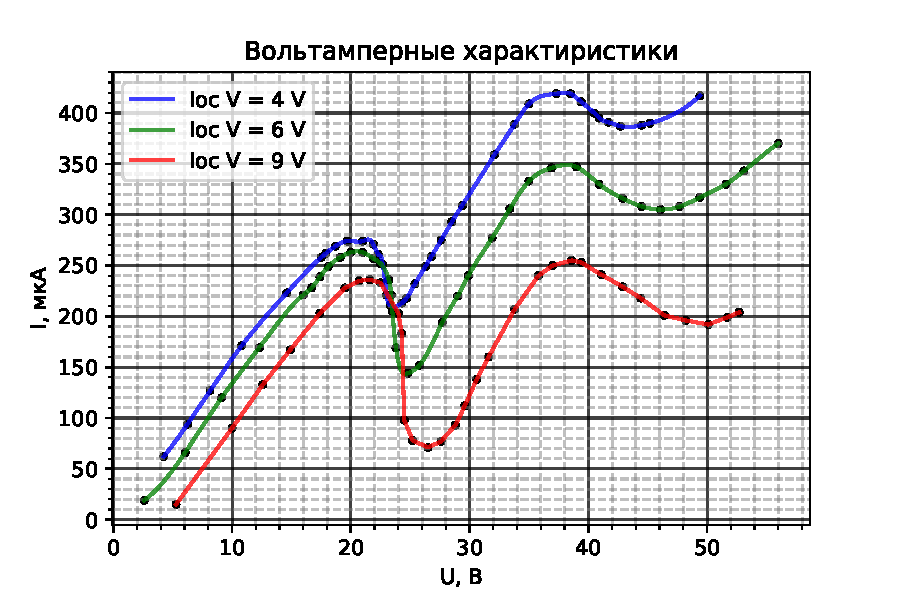
\includegraphics[width=0.6\textheight]{VAC.pdf}
        \caption{ВАХ для трех значений запирающего напряжения}
        \label{fig:VAC}
    \end{figure}

\end{document}